\section{Detection Patterns}


Die erste Phase von Fault Tolerance ist Entdeckung. Faults und daraus resultierende Errors müssen erst erkannt werden, bevor Recovery- oder Schadensminderungsaktionen etc. ausgeführt werden können.

Zwei Paare von Konzepten sind dabei wichtig: 'Errors' vs. 'Failures' und 'a priori Wissen' vs. 'Vergleich von redundanten Elementen'.
\begin{figure}[H]
	\centering
	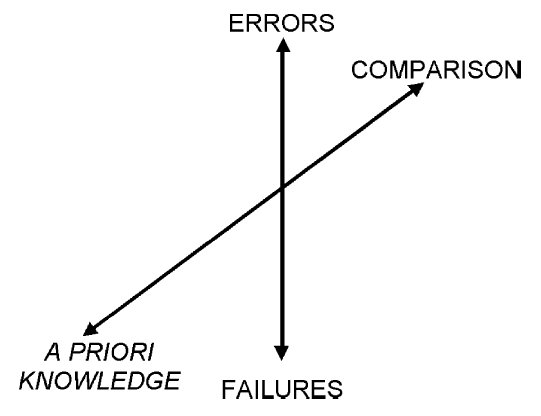
\includegraphics[width=\textwidth]{content/faulttolerance/images/detection_concepts.png}
	\caption{detection concepts}
\end{figure}


\subsection*{'a priori Wissen' vs. 'Vergleich von redundanten Elementen'}


Wir können Wissen über das System und darin geltende Constraints nutzen um zur Laufzeit Zustände, Resultate, Seiteneffekte etc. überprüfen zu können.

Die meisten Patterns nutzen eher den zweiten Ansatz, wie z.B. REDUNDANCY(4).

Ein weiterer Aspekt wäre, dass das Programm selbst in der Lage ist, zu erkennen, dass (und welche) Fehler immer wieder auftauchen und so automatisch Errors und Failures erkennt.

\subsection*{'Errors' vs. 'Failures'}


Das System muss in der Lage sein, sowohl Errors als auch Failures zu erkennen. Wir sind natürlich v.a. an den Errors interessiert, da diese die "Wurzel der Probleme" sind. Bestenfalls finden wir sie, wenn sie noch gar nie im System Schaden anrichten konnten.

\begin{figure}[H]
	\centering
	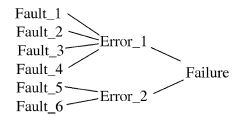
\includegraphics{content/faulttolerance/images/FaultErrorFailureDependency.JPG}
	\caption{Fault Error Failure Dependency}
\end{figure}


\subsection*{Übersicht über die Patterns im folgenden Kapitel}


\begin{figure}
	\centering
	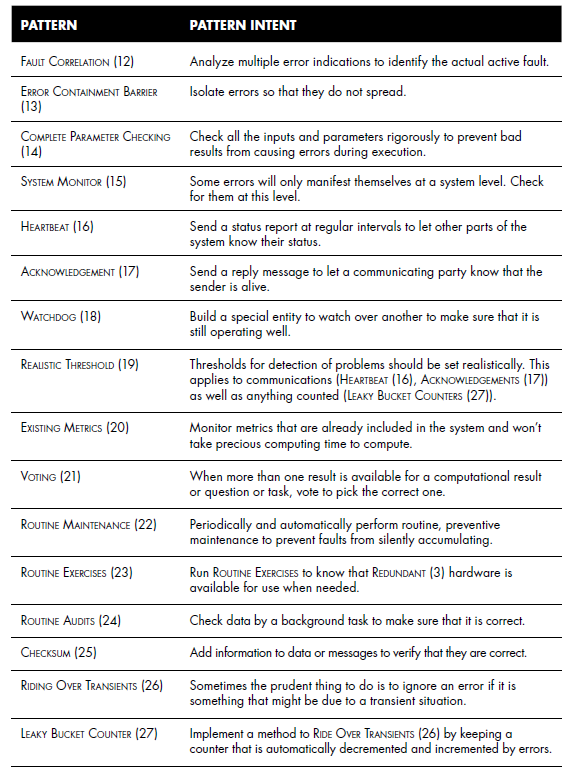
\includegraphics{content/faulttolerance/images/pattern_thumbnails.png}
	\caption{pattern thumbnails}
\end{figure}


\begin{figure}
	\centering
	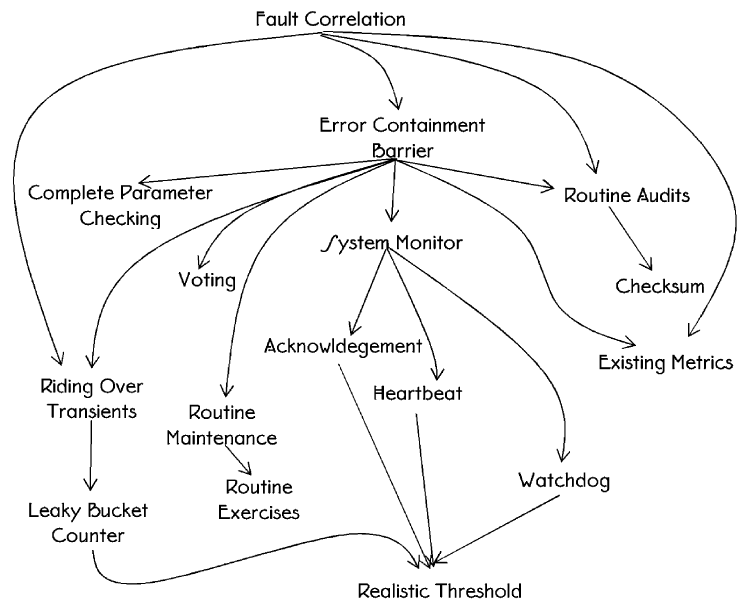
\includegraphics[width=\textwidth]{content/faulttolerance/images/pattern_map.png}
	\caption{pattern map}
\end{figure}


